\section{Aufgaben (TiK)}
Wesentliche Fragestellungen, die in diesem Kapitel gelöst werden sollen, sind auf der einen Seite, welche vorhandene IT-Systeme bereits zentral Verwendung finden und auf der anderen Seite, wie Informationen bereits repräsentiert werden. Des weiteren soll in dieser Analyse Aufschluss darüber gegeben werden, ob ein Informationsmanagement bereits an der Hochschule betrieben wird und wie Informationen bereits zentral zur Verfügung gestellt werden.  
Bei der Hochschule Emden-Leer handelt es sich um eine kleine Hochschule mit aktuell 4626 eingeschriebenen Studierenden. Den größten Anteil machen die 4303 Studenten vor Ort aus.\footnote{\url{http://www.hs-emden-leer.de/fileadmin/user_upload/Einrichtungen/ZDF/Studierende/JV_Stud_20142.pdf}} Es sind 396 Mitarbeiter beschäftigt, wobei 107 Professuren sind.\footnote{\url{https://www.hs-emden-leer.de/no_cache/hochschule/zahlen-daten-fakten.html}}

Ein Hauptbestandteil dieses Kapitels ist der Prozess der Sammlung, Selektion und Prüfung von Fragestellungen, welche die Grundlage für ein Experteninterview bilden. Im Rahmen dieser Ausarbeitung wurde sich für die Verwendung eines Experteninterviews entschieden, da hier die Zielgruppe ein Spezialist aus dem Fachbereich ist. In diesem Fall ist der Interviewte der Leiter des Hochschulrechenzentrums der Hochschule Emden/Leer, Herr Günter Müller. Dieses Interview wurde durch die Studierenden Tina Koppermann, Marc Enders, der betreuenden Professorin Frau Prof. Dr. Krüger-Basener mit Herrn Günter Müller durchgeführt. 

Es wurde bei der Erstellung dieses Experteninterviews auf die Methodik des SPSS-Prinzipes verstärkt reflektiert. Dem SPSS-Prinzip nach Helfferich\footnote{\cite{helfferich_2009}} liegt folgendes Vorgehen zur Grunde:
\begin{enumerate}
	\item Sammeln
	\item Prüfen
	\item Selektieren
	\item Subsumieren		
\end{enumerate}
Mit Hilfe dieses Prinzips zur qualitativen Datenerhebung wurden im ersten Schritt Fragen gesammelt. Diese konnten von allen Kursteilnehmern in einem zur Verfügung gestellten Online-Dokument eingesehen und editiert werden. Bei der Sammlung der Fragen sind insgesamt 62 Fragestellungen zu unterschiedlichen Schwerpunkten aufgenommen worden(siehe Abbildung \ref{fig_auszug_fragen_sammeln}).

\begin{figure}[h!]
	\centering
	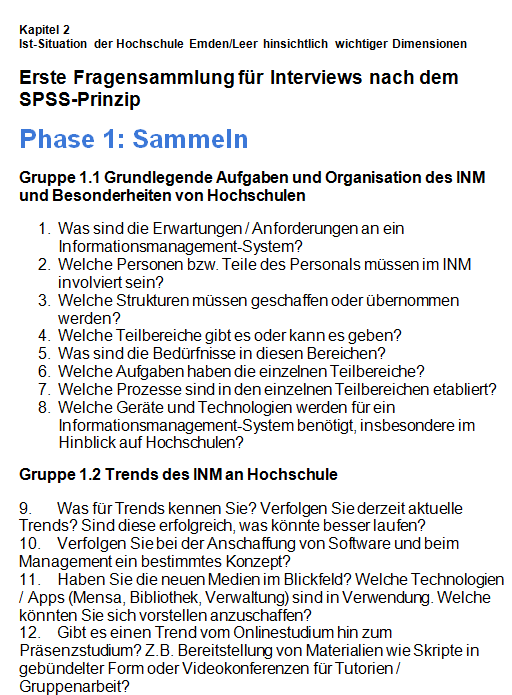
\includegraphics[width=10cm]{kapitel/gruppe2/bilder/auszug_fragen}
	\caption{Auszug der gesammelten Fragen}
	\label{fig_auszug_fragen_sammeln}
\end{figure}
Nach erfolgter Sammlung aller Fragen folgte im zweiten Schritt die Prüfung dieser. Hierbei wurden reine Informationsfragen aussortiert. Nach der erfolgreichen Prüfung der Fragen folgte im nächsten Schritt die Selektion dieser. Die Fragestellungen wurden nach Themengebieten kategorisiert. 

Im letzten Schritt, dem Subsumieren des SPSS-Prinzips, wurde für jedes Themengebiet eine Erzählaufforderung gefunden und der Interviewleitfaden entsprechend dieser gegliedert. Mit Hilfe eines Farbcodes (siehe Abbildung \ref{fig_farbcode_SPSS}) wurden die Fragen entsprechend nach Erzählaufforderung, Checkliste, konkreter Frage und Aufrechterhaltungsfrage farblich markiert und anschließend einsortiert (siehe Abbildung \ref{fig_sortierung_fragentyp}).

\begin{figure}[h!]
	\centering
	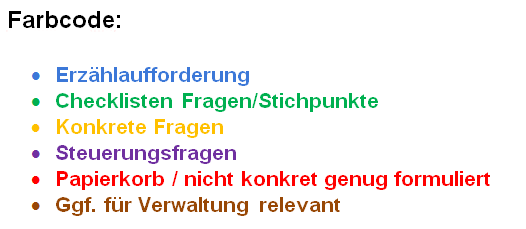
\includegraphics[width=10cm]{kapitel/gruppe2/bilder/farbcode_spss}
	\caption{angewandter Farbcode für das SPSS-Prinzip}
	\label{fig_farbcode_SPSS}
\end{figure}

\begin{figure}[h!]
	\centering
	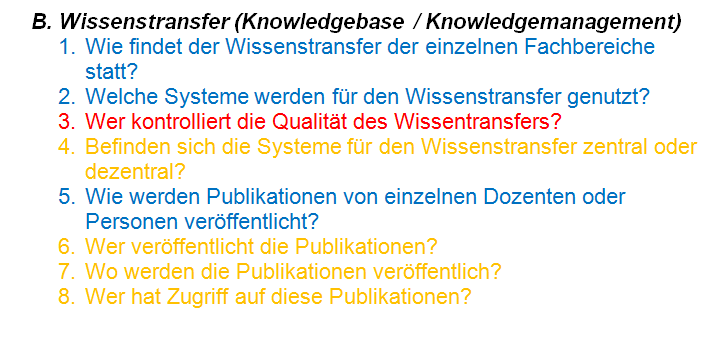
\includegraphics[width=10cm]{kapitel/gruppe2/bilder/sortierung_fragentyp}
	\caption{Sortierung der Fragen nach Fragentyp}
	\label{fig_sortierung_fragentyp}
\end{figure}

Diese Subsumtion wurde mit Hilfe des Anwendungsprogramms Microsoft Excel entsprechend visualisiert. Als Endergebnis ist ein Interviewleitfaden entstanden, der in acht unterschiedliche Themenbereiche unterteilt wurde  (siehe Abbildung: \ref{fig_auszug_interviewleitfaden}).

\begin{figure}[h!]
	\centering
	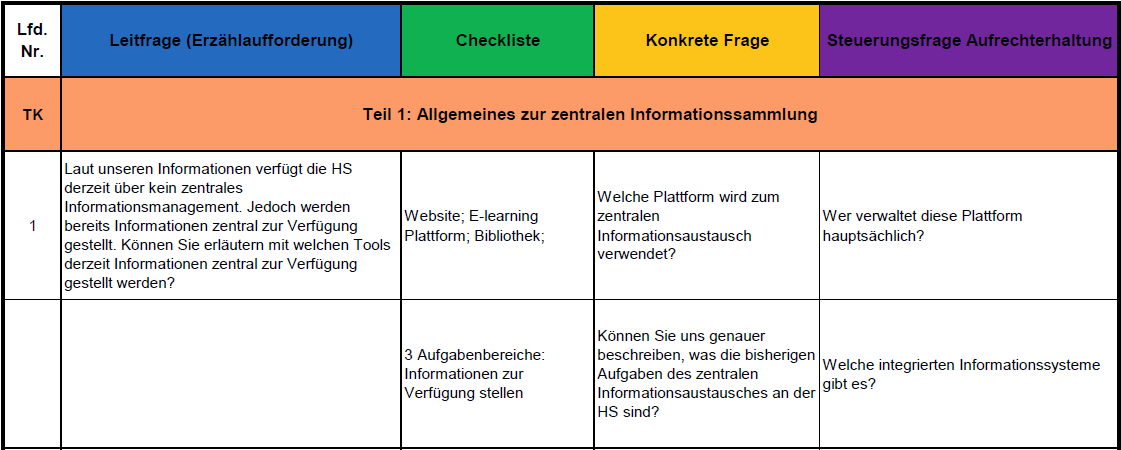
\includegraphics[width=10cm]{kapitel/gruppe2/bilder/auszug_leitfaden}
	\caption{Auszug des Interviewleitfadens}
	\label{fig_auszug_interviewleitfaden}
\end{figure}

An einem festgelegtem Interviewtermin ist mit Hilfe von diesem Leitfaden das Experteninterview mit Herrn Günter Müller durchgeführt worden. Dieses Interview fand mit der Online Video Plattform „Adobe Connect“ statt und wurde mit Zustimmung von Herrn Müller digital aufgezeichnet. Im Anschluss an das Experteninterview wurde in der ersten Phase die digitale Aufzeichnung auf wichtige inhaltliche Aspekte analysiert. 

In der zweiten Phase wurde durch Transkription die zur Verfügung gestellte Aufzeichnung, mit Hilfe der Applikation „Microsoft Word“, überführt, um die im Interview erhaltenen Informationen besser verarbeiten zu können.

\begin{figure}[h!]
	\centering
	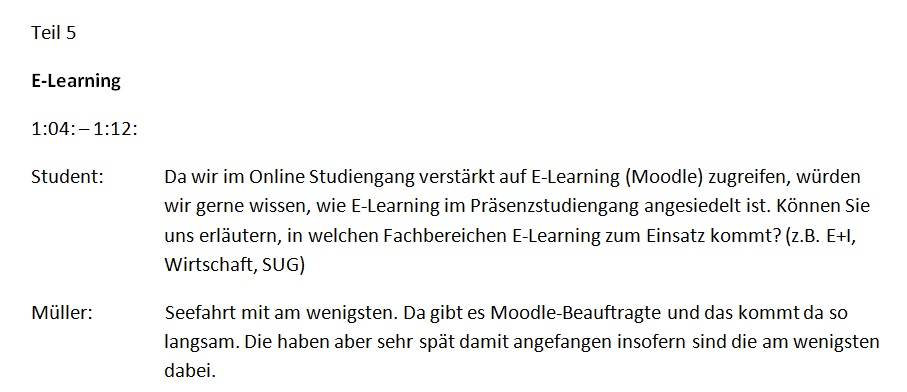
\includegraphics[width=10cm]{kapitel/gruppe2/bilder/E-Learning_Transkription}
	\caption{Transkription: E-Learning}
	\label{fig_E-Learning_Transkription}
\end{figure}

In der dritten und letzten Phase wurden mit Hilfe des Tools „XMind6“ zu jedem Themenbereich ein entsprechendes Mindmap generiert, um somit bei der Recherche schneller auf Besonderheiten eingehen zu können  (siehe Abbildung \ref{fig_E-Learning_MM}).

\begin{figure}[h!]
	\centering
	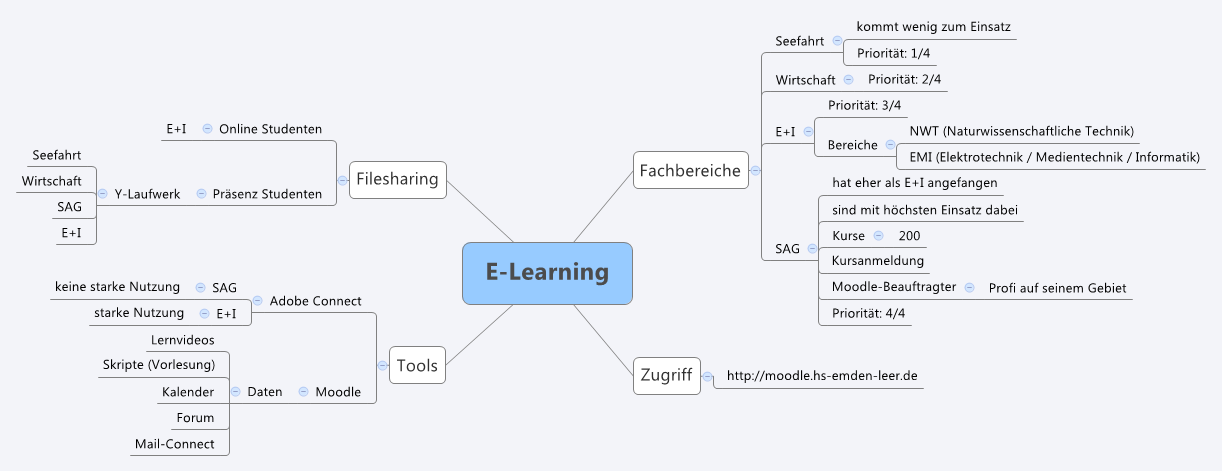
\includegraphics[width=10cm]{kapitel/gruppe2/bilder/E-Learning_MM}
	\caption{Mindmap: E-Learning}
	\label{fig_E-Learning_MM}
\end{figure}

Die Ergebnisse dieser Analyse werden in den folgenden Kapiteln detaillierter beschrieben. 
